\documentclass[usenames,dvipsnames]{beamer}
\usetheme{Copenhagen}
\useinnertheme{circles}
\useoutertheme{split}
\setbeamertemplate{itemize items}[triangle]
\beamertemplatenavigationsymbolsempty

\usepackage[english]{babel}
\usepackage[utf8]{inputenc}
\usepackage[T1]{fontenc}
\usepackage{lmodern}
\usepackage{textcomp}
\usepackage{tikz}
\usepackage{eso-pic}
\usepackage{amsmath}
\usepackage{bookmark}
\usepackage{ifthen}
\usepackage{booktabs}
\usepackage{array}
\usepackage{multirow}
\usepackage{multicol}
\usepackage{fontawesome}
\usepackage{graphicx}
\usepackage{hyperref}
\usepackage{listings}
\usepackage{fancyvrb}
\usepackage{ulem}
\usepackage{xcolor}
%\usepackage{pgfpages}

\usetikzlibrary{calc}
\usetikzlibrary{fit}

\definecolor{logogreen1}{RGB}{52,166,77}
\definecolor{logogreen2}{RGB}{73,180,58}
\definecolor{logogreen3}{RGB}{117,200,44}
\definecolor{logogreen4}{RGB}{157,212,31}
\definecolor{logogreen5}{RGB}{67,149,55}
\definecolor{logogreen6}{RGB}{35,144,63}
\definecolor{titlegreen}{RGB}{72,147,65}
\definecolor{textgrey}{RGB}{138,140,142}
\definecolor{bulletsgreen}{RGB}{171,208,55}

\definecolor{pblue}{rgb}{0.13,0.13,1}
\definecolor{pgreen}{rgb}{0,0.5,0}
\definecolor{pred}{rgb}{0.9,0,0}
\definecolor{pgrey}{rgb}{0.46,0.45,0.48}
\definecolor{pbrown}{RGB}{128,128,0}

\setbeamercolor*{structure}{fg=bulletsgreen}
\setbeamercolor*{palette primary}{fg=white,bg=logogreen3}
\setbeamercolor*{palette quaternary}{fg=white,bg=logogreen6}
\setbeamercolor*{normal text}{fg=textgrey, bg=white}
\setbeamercolor*{titlelike}{fg=titlegreen, bg=white}
\setbeamercolor*{block title}{fg=white, bg=logogreen1}

\makeatletter
\renewcommand{\@makefnmark}{\hbox{\textsuperscript{\tiny{\@thefnmark}}}}
\makeatother

\newenvironment<>{mydef}[1]{%
  \setbeamercolor{block title}{fg=white,bg=logogreen6}%
  \begin{block}#2{#1}}
{\end{block}}

\newenvironment<>{operations}
	{\begin{block}{Operations}{#1}}
	{\end{block}}


\setcounter{tocdepth}{4}
\newboolean{subsectiontoc}
\setboolean{subsectiontoc}{true}
\setbeamerfont{subsubsection in toc}{size=\tiny}
\setbeamertemplate{subsubsection in toc}{\leavevmode\leftskip=3em\inserttocsubsubsection\par}
%\addtobeamertemplate{footline}{\hfill\insertframenumber/\inserttotalframenumber\newline}{}

\AtBeginSection[]
{
  \begin{frame}
  \frametitle{Outline}
  \tiny{\tableofcontents[currentsection,subsubsectionstyle=hide]}
  \end{frame}
}
\AtBeginSubsection[]
{
	\ifthenelse{\boolean{subsectiontoc}}{
		\begin{frame}
			\frametitle{Outline}
			\tiny{\tableofcontents[sectionstyle=show/shaded,currentsubsection,subsubsectionstyle=hide]}
		\end{frame}
	}{
		\begin{frame}
			\frametitle{Outline}
			\tiny{\tableofcontents[sectionstyle=show/shaded,currentsubsection,subsubsectionstyle=show]}
		\end{frame}
	}
}

\newcommand{\deeptocsubsection}[1]{
  \setboolean{subsectiontoc}{false}
  \subsection{#1}
  \setboolean{subsectiontoc}{true}
}

\newcommand\AtPagemyUpperLeft[1]{\AtPageLowerLeft{%
\put(\LenToUnit{0mm},\LenToUnit{3.38mm}){#1}}}%
\AddToShipoutPictureFG{%
  \AtPagemyUpperLeft{{
\includegraphics[width=.5cm,keepaspectratio]{r.png}}}
}

\newcolumntype{C}[1]{>{\centering\let\newline\\\arraybackslash\hspace{0pt}}m{#1}}
\newcolumntype{L}[1]{>{\raggedright\let\newline\\\arraybackslash\hspace{0pt}}m{#1}}
\newlength{\myl}
\newlength{\myll}
\renewcommand{\arraystretch}{1.3}

\makeatletter
\newcommand\colorwave[1][red]{\bgroup \markoverwith{\lower3.5\p@\hbox{\sixly \textcolor{#1}{\char58}}}\ULon}
\font\sixly=lasy6 % does not re-load if already loaded, so no memory problem.
\makeatother

\lstset{
	language=Java,
  commentstyle=\color{pgrey},
  keywordstyle=\color{pblue},
  stringstyle=\color{pgreen},
	frame=tblr
	backgroundcolor=\color{logogreen6},
	extendedchars=true,
	showstringspaces=false,
	showspaces=false,
	tabsize=2,
	breaklines=true,
	showtabs=false,
	captionpos=b,
	basicstyle=\ttfamily\scriptsize\color{black},
	basewidth=0.5em,
	escapechar=\%,
  moredelim=[il][\textcolor{pbrown}]{$$}
}

\makeatletter
\newenvironment{SmallListing}[1][]
  {\lstset{#1}\VerbatimEnvironment\begin{VerbatimOut}{VerbEnv.tmp}}
  {\end{VerbatimOut}\settowidth\@tempdima{%
    \lstinputlisting{VerbEnv.tmp}}
  \minipage{\@tempdima}\lstinputlisting{VerbEnv.tmp}\endminipage}    
\makeatother

\title[{\makebox[.45\paperwidth]{Nieuwigheden in Java 8\hfill}}]{Nieuwigheden Java 8}
\author[{\makebox[.45\paperwidth]{\hfill Maarten Dhondt}}]{Maarten Dhondt}
\institute{Realdolmen}
\date{October 25, 2018}

%\setbeameroption{show notes on second screen=right}

\begin{document}

\frame{\titlepage}

{
\usebackgroundtemplate{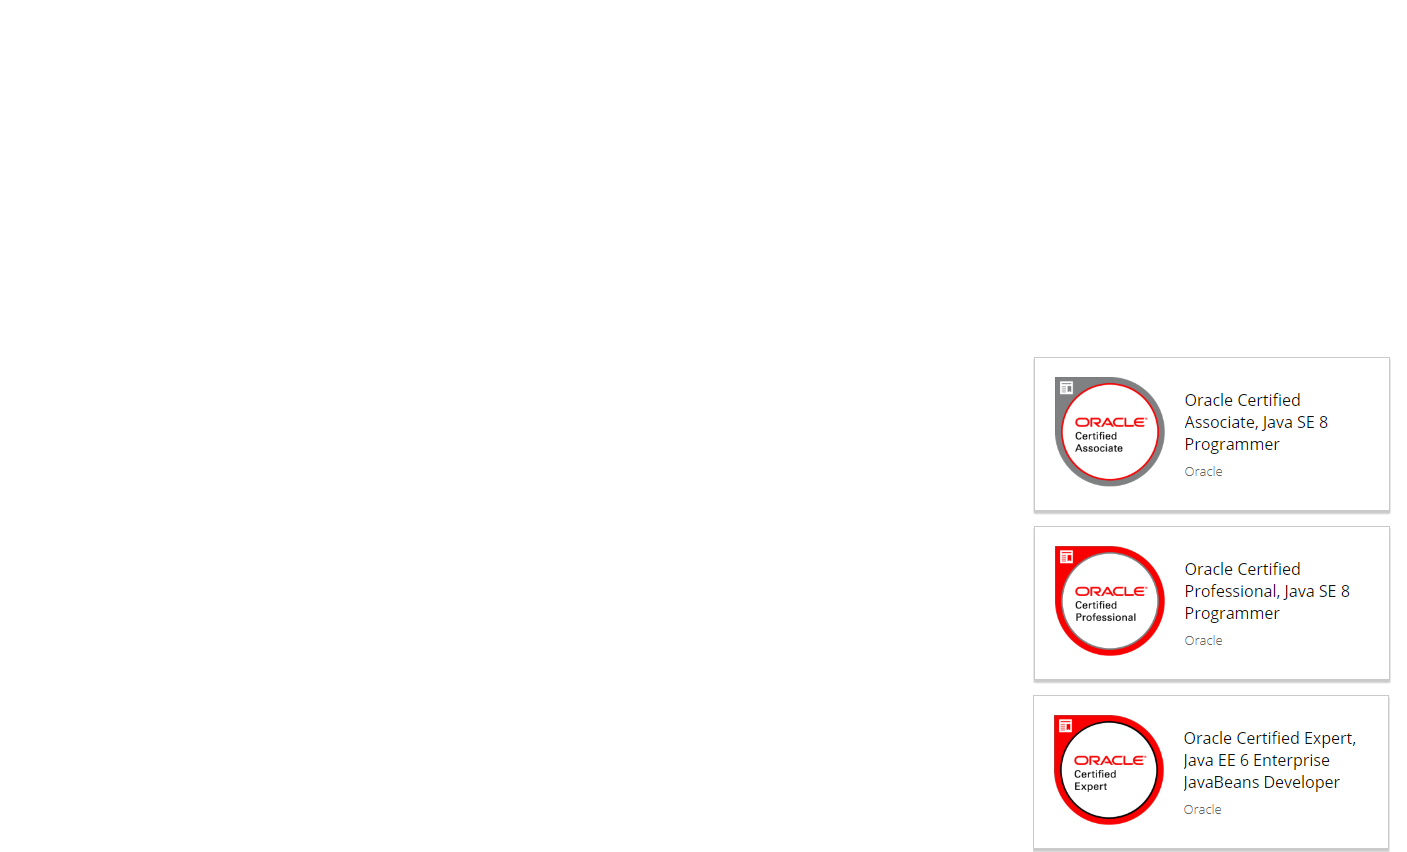
\includegraphics[width=\paperwidth]{badges}}
\begin{frame}
	\frametitle{Wie ben ik?}
	\begin{itemize}
		\item Master in de ingenieurswetenschappen: computerwetenschappen (KUL)
		\begin{itemize}
			\item Computationele informatica
		\end{itemize}
		\item Master in Management (KUL)
		\item Software engineer @ Realdolmen sinds 2015
		\item Projecten: 
		\begin{itemize}
			\item Infrastructuur planning @ Infrabel
			\item API platform @ Proximus
		\end{itemize}
		\item Contact:
		\begin{itemize}
			\item \scalebox{.85}{\faEnvelope}~\href{mailto:maarten.dhondt@realdolmen.com}{maarten.dhondt@realdolmen.com}
			\item \faLinkedinSquare~\href{https://www.linkedin.com/in/maartendhondt/}{maartendhondt}
			\item \faGithubSquare~\href{https://github.com/MDhondt/}{MDhondt}
		\end{itemize}
	\end{itemize}
\end{frame}
}

\title[{\makebox[.45\paperwidth]{Nieuwigheden in Java 8\hfill\insertframenumber/\inserttotalframenumber}}]{Nieuwigheden in Java 8}
\author[{\makebox[.45\paperwidth]{https://github.com/MDhondt/java8-presentation}}]{Maarten Dhondt}

\begin{frame}
  \frametitle{Outline}
  \tiny{\tableofcontents}
\end{frame}

\author{Maarten Dhondt}

\section{Java 8}

\subsection{Interfaces}

\begin{frame}
	\frametitle{Interfaces}
	
	\begin{itemize}
		\item Een interface gelijkt op een klasse, maar bevat enkel methoden en attributen. Interfaces hebben geen geïmplementeerde methoden, maar enkel de signatuur.
		\begin{itemize}
			\item Implementaties hebben dezelfde signatuur maar return type kan een subklasse zijn.
			\item Implementaties gooien geen andere checked exceptions dan diegene uit de interface.
			\item Abstracte klassen kunnen methoden implementeren, maar niet vereist.
		\end{itemize}
	\end{itemize}
\end{frame}

\begin{frame}[fragile]
	\frametitle{Interfaces}
	Implementatie zelfde signatuur maar return type kan subklasse zijn.
	\begin{lstlisting}
public abstract class Transaction {}
	\end{lstlisting}
	\begin{lstlisting}
public class BankTransaction extends Transaction {}
	\end{lstlisting}
	\hrule\vspace{.2cm}
	\begin{lstlisting}
public interface Transactionable {
    Transaction doTransaction();
}
	\end{lstlisting}
	\begin{lstlisting}
public class BankTranserService implements Transactionable {
    @Override
    public BankTransaction doTransaction() {
        ...
    }
}
	\end{lstlisting}
\end{frame}

\begin{frame}[fragile]
	\frametitle{Interfaces}
	Implementatie gooit geen andere checked exceptions.
	\begin{lstlisting}
public interface ExceptionThrowingInterface {
    void doStuff() throws IOException;
}
	\end{lstlisting}
	\begin{lstlisting}
public class ExceptionThrower implements ExceptionThrowingInterface {
    @Override
    public void doStuff() throws IOException, %\colorwave{ReflectionException}% {
				// 'doStuff()' in 'ExceptionThrower' clashes with 'doStuff()' in 'ExceptionThrowingInterface'; overriden method does not throw 'javax.management.ReflectionException'
    }
}
	\end{lstlisting}
\end{frame}

\begin{frame}[fragile]
	\frametitle{Interfaces}
	Abstracte klasse kan methode implementeren, maar niet vereist
	\begin{lstlisting}
public interface Moveable {
    void move();
}
	\end{lstlisting}
	\begin{lstlisting}
public abstract class Furniture implements Moveable {}
	\end{lstlisting}
	\begin{lstlisting}
public class Chair extends Furniture {
    @Override
    public void move() {
        System.out.println("Moved chair");
    }
}
	\end{lstlisting}
\end{frame}

\begin{frame}
	\frametitle{Interfaces}
	\begin{itemize}
		\item Java 8 introduceert \texttt{default} methoden.
		\begin{itemize}
			\item Wat? Een implementatie in de interface.
			\item Waarom? Optionele methoden
			\item Waarom? Gedrag overerving van meerder klassen.
		\end{itemize}
		\item Vorige regels blijven (uiteraard) geldig.
	\end{itemize}
\end{frame}

\begin{frame}[fragile]
	\frametitle{Interfaces}
	\begin{itemize}
		\item Voorbeeld van een \texttt{default} methode.
	\begin{lstlisting}
public interface Animal {

		void eat();
		
		void move();
		
		void sleep();
		
    default void blinkEyes() {
        System.out.println("Blink");
    }
}
	\end{lstlisting}
	\end{itemize}
\end{frame}

\begin{frame}[fragile]
	\frametitle{Interfaces}
	\begin{itemize}
		\item \texttt{default} methoden: optionele methoden.
	\begin{lstlisting}
public interface Collection<E> extends Iterable<E> {

    default boolean removeIf(Predicate<? super E> filter) {
        Objects.requireNonNull(filter);
        boolean removed = false;
        final Iterator<E> each = iterator();
        while (each.hasNext()) {
            if (filter.test(each.next())) {
                each.remove();
                removed = true;
            }
        }
        return removed;
    }
				
}
	\end{lstlisting}
	\end{itemize}
\end{frame}

\begin{frame}
	\frametitle{Interfaces}
	
	Java 8 introduceert ook SAM (Single Abstract Method) interfaces die we functionele interfaces noemen.
	\begin{itemize}
		\item Interface moet exact 1 abstracte methode hebben.
		\item Met of zonder \texttt{@FunctionalInterface} annotatie.
	\end{itemize}
	Kunnen gebruikt worden in lambda expressies en method references
\end{frame}

\begin{frame}[fragile]
	\frametitle{Interfaces}
	
	\begin{lstlisting}
package java.lang;

$$@FunctionalInterface
public interface Runnable {
    public abstract void run();
}
	\end{lstlisting}
	\begin{lstlisting}
public class Main {
    public static void main(String[] args) {
        ExecutorService executor = Executors.newSingleThreadExecutor();
        executor.submit(() -> {
            System.out.println(Thread.currentThread().getName());
        });
    }
}
	\end{lstlisting}
\end{frame}

\subsection{Lambda expressies}

\begin{frame}
	\frametitle{Lambda expressies}
	
	Lambda expressies zijn een nieuwe en belangrijke functie uit Java 8 die:
	\begin{itemize}
		\item op een duidelijke en bondige manier een interface methode beschrijven in een expressie,
		\item een grote verbetering mogelijk maken van de Collection libraries.
	\end{itemize}
\end{frame}

\begin{frame}[fragile]
	\frametitle{Lambda expressies}
	
	\begin{itemize}
		\item Lambda expressies bieden een oplossing aan de verbose anonieme inner klassen door 5 lijnen code te reduceren naar 1 lijn.
		\item Deze horizontale oplossing, lost het verticale probleem van inner klassen op.
		\item Een lambda expressie bestaat uit 3 delen:
		\begin{itemize}
			\item Argumenten lijst
			\item Pijltje: \texttt{->}
			\item Body
		\end{itemize}
	\end{itemize}
	\begin{lstlisting}
(int x, int y) -> x + y
	\end{lstlisting}
\end{frame}

\begin{frame}[fragile]
	\frametitle{Lambda expressies: syntax}
	Argumenten lijst:
	\begin{itemize}
		\item Kan 0, 1 of meer argumenten zijn,
		\item Types kunnen expliciet gedeclareerd of afgeleid worden,
		\item Argumenten worden tussen haakjes gescheiden door komma's,
		\item Lege haakjes worden gebruikt voor een lege argumenten lijst,
		\item Bij 1 argument met een afgeleid type, zijn haakjes niet nodig.
	\end{itemize}
\end{frame}

\begin{frame}[fragile]
	\frametitle{Lambda expressies: syntax}
	Body:
	\begin{itemize}
		\item Kan 0, 1 of meer statements bevatten,
		\item Bij 1 statement kunnen accolades en \texttt{return} keywoord weggelaten worden,
		\item Bij meerdere statements moeten die tussen accolades geplaatst worden en is een \texttt{return} statement verplicht wanneer er iets moet gereturned worden.
	\end{itemize}
\end{frame}

\begin{frame}[fragile]
	\frametitle{Lambda expressies: syntax}
	Voorbeelden:
	\begin{lstlisting}
n -> n %\%% 2 != 0;

(char c) -> c == 'y';

(x, y) -> x + y;

(int a, int b) -> a * a + b * b;

() -> 42

() -> { return 3.14 };

(String s) -> { System.out.println(s); };

() -> { System.out.println("Hello World!"); };
	\end{lstlisting}
\end{frame}

\begin{frame}[fragile]
	\frametitle{Lambda expressies}
	\begin{lstlisting}
$$@FunctionalInterface
public interface LambdaInterface {
  String doStuff(Integer x, String y);
}
	\end{lstlisting}
	\begin{lstlisting}
public class Main {
  public static void main(String[] args) {
    LambdaInterface anonymousImpl = new LambdaInterface() {
      @Override
      public String doStuff(Integer x, String y) {
        return "x=" + x + ",y=" + y;
    }};

    LambdaInterface lambdaImpl = (x, y) -> "x=" + x + ",y=" + y;

    System.out.println(anonymousImpl.doStuff(5, "Abc"));
    System.out.println(lambdaImpl.doStuff(5, "Abc"));
}}
	\end{lstlisting}
\end{frame}

\begin{frame}[fragile]
	\frametitle{Method references}
	
	Method references zijn gelinkt aan lambda expressies:
	\begin{itemize}
		\item Wordt gebruikt om bestaande methode definities te hergebruiken
		\item Wordt doorgegeven op dezelfde manier als lambda expressies
	\end{itemize}
	\begin{lstlisting}
Object::methodName
	\end{lstlisting}
	\begin{itemize}
		\item Het object of de klasse die een methode bevat wordt voor de dubbele dubbelpunt geplaatst.
		\item De naam van de methode komt erna. Zonder argumenten.
	\end{itemize}
\end{frame}

\begin{frame}[fragile]
	\frametitle{Method references}
	
	\begin{itemize}
		\item Referentie naar een static method
		\begin{itemize}
			\item [$\lambda$] \texttt{(args) -> ClassName.staticMethodName(args)}
			\item [MR] \texttt{ClassName::staticMethodName}
		\end{itemize}
		\item Referentie naar instantie methode van een bestaand object
		\begin{itemize}
			\item [$\lambda$] \texttt{(args) -> object.instanceMethodName(args)}
			\item [MR] \texttt{object::instanceMethodName}
		\end{itemize}
		\item Referentie naar instantie methode van een arbitrair object
		\begin{itemize}
			\item [$\lambda$] \texttt{(arg0,rest) -> arg0.instanceMethodName(rest)}
			\item [MR] \texttt{ClassName::instanceMethodName}
		\end{itemize}
		\item Referentie naar een constructor
		\begin{itemize}
			\item [$\lambda$] \texttt{(args) -> new ClassName(args)}
			\item [MR] \texttt{ClassName::new}
		\end{itemize}
	\end{itemize}
\end{frame}

\begin{frame}[fragile]
	\frametitle{Lambda expressies}
	
	\begin{itemize}
		\item Lambda expressies en vooral method references hebben wat oefening nodig alvorens er vlug meer overweg te kunnen.
		\item Java 8 introduceert een nieuwe \texttt{package} \texttt{java.util.function} met 43 functionele interfaces waarvan een aantal een belangrijk deel uitmaken van uw dagdagelijkse code.
	\end{itemize}
\end{frame}

\begin{frame}[fragile]
	\frametitle{\texttt{java.util.function}}
	
	4 categorieën:
	\begin{itemize}
		\item \texttt{Supplier}
		\item \texttt{Consumer}
		\begin{itemize}
			\item \texttt{BiConsumer}
		\end{itemize}
		\item \texttt{Predicate}
		\begin{itemize}
			\item \texttt{BiPredicate}
		\end{itemize}
		\item \texttt{Function}
		\begin{itemize}
			\item \texttt{BiFunction}
			\item \texttt{UnaryOperator}
			\item \texttt{BinaryOperator}
		\end{itemize}
	\end{itemize}
\end{frame}

\begin{frame}[fragile]
	\frametitle{Suppliers}
	
	\begin{itemize}
		\item Een \texttt{Supplier} neemt geen argumenten
		\item Een \texttt{Supplier} levert een waarde (via zijn \texttt{get()} methode)
	\end{itemize}
	
	\begin{lstlisting}
static void display(Supplier<Integer> suppl) {
		System.out.println(suppl.get());
}
	\end{lstlisting}
	\begin{lstlisting}
display(() -> 10);
display(() -> 100);
	\end{lstlisting}
\end{frame}

\begin{frame}[fragile]
	\frametitle{Consumers}
	
	\begin{itemize}
		\item Een \texttt{Consumer} neemt argumenten
		\item Een \texttt{Consumer} returned \texttt{void} (via zijn \texttt{accept()} methode)
	\end{itemize}
	
	\begin{lstlisting}
static void display(int value) {
		switch (value) {
				case 1:  System.out.println("Value is 1");
								 return;
				default: System.out.println("Value != 1");
								 return;
		}
}
	\end{lstlisting}
	\begin{lstlisting}
Consumer<Integer> consumer = x -> display(x - 1);
consumer.accept(2);
	\end{lstlisting}
\end{frame}

\begin{frame}[fragile]
	\frametitle{Predicates}
	
	\begin{itemize}
		\item Een \texttt{Predicate} neemt argumenten en returned een boolean
	\end{itemize}
	\begin{lstlisting}
public interface Collection<E> extends Iterable<E> {
    default boolean removeIf(Predicate<? super E> filter) {
        Objects.requireNonNull(filter);
        boolean removed = false;
        final Iterator<E> each = iterator();
        while (each.hasNext()) {
            if (filter.test(each.next())) {
                each.remove();
                removed = true;
        }}
        return removed;
}}
	\end{lstlisting}
	\begin{lstlisting}
List<String> animals = Arrays.asList("cat", "dog", "cheetah", "deer");

animals.removeIf(element -> element.startsWith("c"));
	\end{lstlisting}
\end{frame}

\begin{frame}
	\frametitle{Java Functional Interface Naming Guide by Esko Luontola}
	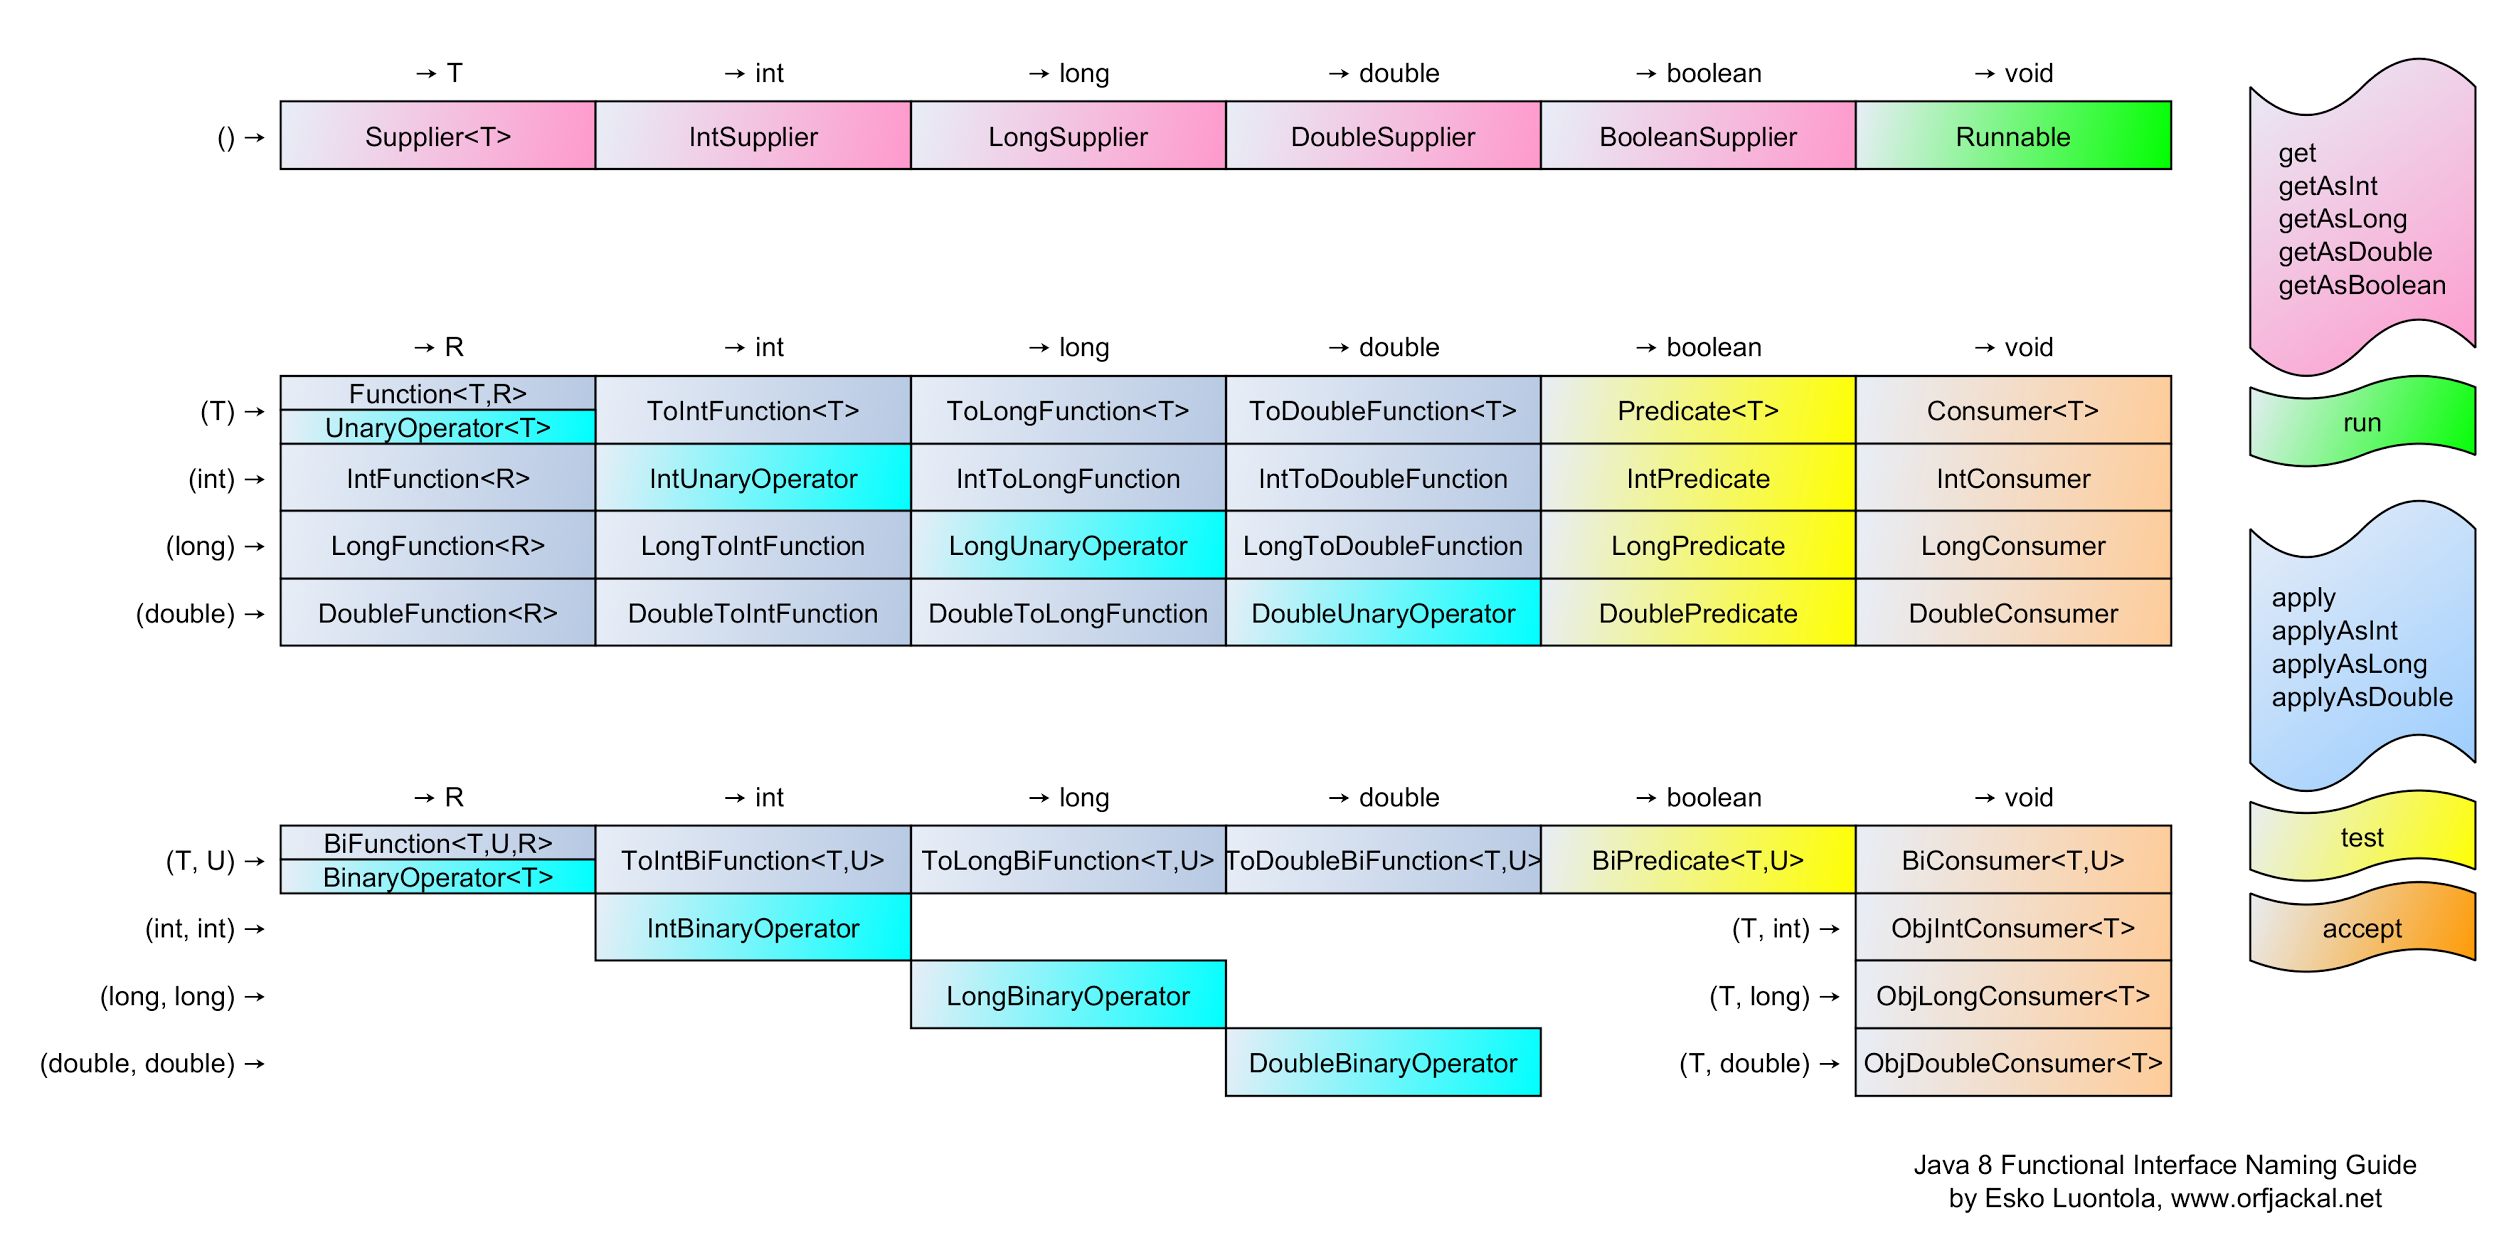
\includegraphics[width=.83\paperwidth]{fi-guide}
\end{frame}

\subsection{Streams}

\begin{frame}
	\frametitle{Streams}
	Wat is een \texttt{Stream}? --- een object
	\begin{itemize}
		\item waarop operaties mogelijk zijn,
		\item dat geen data bijhoudt (in tegenstelling to \texttt{Collection})
		\item dat de data waarop het werkt niet veranderd
		\item dat enorme hoeveelheden data kan verwerken in 1 statement
		\item dat algoritmisch geöptimaliseerd is om data in parallel te verwerken.
	\end{itemize}
\end{frame}

\begin{frame}
	\frametitle{Streams}
	Waarin verschillen Streams van Collections?
	\begin{itemize}
		\item Collections houden zich bezig met het efficiënte management en toegang tot data.
		\item Streams bieden geen rechtstreekse functionaliteit om data aan te passen, maar zijn gemaakt om op een declaratieve manier operaties op de data te omschrijven.
		\item Streams zijn:
		\begin{itemize}
			\item geen opslag of datastructuur
			\item functioneel by design (een resultaat produceren zonder de bron data aan te passen)
			\item Lazy
			\item Optioneel gebonden
		\end{itemize}
	\end{itemize}
\end{frame}

\begin{frame}
	\frametitle{Streams}
	Hoe bekom ik zo'n Stream?
	\begin{itemize}
		\item \texttt{java.util.Collection} heeft 2 nieuwe default methoden
		\begin{itemize}
			\item \texttt{default Stream<E> stream()}
			\item \texttt{default Stream<E> parallelStream()}
		\end{itemize}
		\item \texttt{java.util.stream.Stream} heeft enkele static methoden
		\begin{itemize}
			\item \texttt{public static<T> Stream<T> of(T... values)}
			\item \texttt{public static<T> Stream<T> iterate(final T seed, final UnaryOperator<T> f)}
			\item \texttt{public static<T> Stream<T> generate(Supplier<T> s)}
		\end{itemize}
	\end{itemize}
\end{frame}

\begin{frame}
	\frametitle{Stream non-terminal operaties}
	\begin{itemize}
		\item \texttt{Stream<T> filter(Predicate<T> predicate);}
		\item \texttt{Stream<R> map(Function<T, R> mapper);}
		\item \texttt{Stream<R> flatMap(Function<T, Stream<R>> mapper);}
		\item \texttt{Stream<T> distinct();}
		\item \texttt{Stream<T> peek(Consumer<T> action);}
		\item \texttt{Stream<T> limit(long maxSize);}
		\item \texttt{Stream<T> skip(long n);}
	\end{itemize}
\end{frame}

\begin{frame}
	\frametitle{Stream terminal operaties}
	\begin{itemize}
		\item \texttt{void forEach(Consumer<T> action);}
		\item \texttt{T reduce(T iden, BinaryOperator<T> accumulator);}
		\item \texttt{R collect(Collector<T, A, R> collector);}
		\item \texttt{Optional<T> min(Comparator<T> comparator);}
		\item \texttt{Optional<T> max(Comparator<T> comparator);}
		\item \texttt{long count();}
		\item \texttt{boolean anyMatch(Predicate<T> predicate);}
		\item \texttt{boolean allMatch(Predicate<T> predicate);}
		\item \texttt{boolean noneMatch(Predicate<T> predicate);}
		\item \texttt{Optional<T> findFirst();}
		\item \texttt{Optional<T> findAny();}
	\end{itemize}
\end{frame}

\begin{frame}[fragile]
	\frametitle{Stream voorbeelden}
	Als in de volgende voorbeelden de klasse \texttt{Person} gebruikt wordt, dan hebben we het over:
	\begin{lstlisting}
public class Person {
	
	private String name;
	private Integer age;
	private String country;
	private Map<Person, String> relationshipsByPerson;
	
	public String getName() { return name; }
	public Integer getAge() { return age; }
	public String getCountry() { return country; }
	public Map<Person, String> getConnections() { 
	  return relationshipsByPerson;
	}
}
	\end{lstlisting}
\end{frame}

\begin{frame}[fragile]
	\frametitle{Stream voorbeelden}
	Hebben we gegevens van volwassen mensen uit België?
	\begin{lstlisting}
public static boolean hasBelgianAdults(Collection<Person> people) {
  return people.stream()
               .filter(person -> person.getAge() >= 18)
               .filter(person -> person.getCountry().equals("Belgium"))
               .collect(Collectors.toList())
               .size() > 0;
}
	\end{lstlisting}
	\begin{lstlisting}
return people.stream()
             .filter(person -> person.getAge() >= 18)
             .filter(person -> person.getCountry().equals("Belgium"))
             .count() > 0;
	\end{lstlisting}
\end{frame}

\begin{frame}[fragile]
	\frametitle{Stream voorbeelden}
	Hebben we gegevens van volwassen mensen uit België?
	\begin{lstlisting}
return people.stream()
             .filter(person -> person.getAge() >= 18)
             .anyMatch(person -> person.getCountry().equals("Belgium"));
	\end{lstlisting}
	\begin{lstlisting}
return people.stream()
             .filter(Objects::nonNull)
             .filter(person -> person.getAge() >= 18)
             .map(Person::getCountry)
             .anyMatch("Belgium"::equalsIgnoreCase);
	\end{lstlisting}
\end{frame}

\begin{frame}[fragile]
	\frametitle{Stream voorbeelden}
	Vind alle personen die een dochter zijn:
	\begin{lstlisting}
public Collection<Person> getDaughters(Collection<Person> people) {
    return people.stream()
                 .filter(Objects::nonNull)
                 .map(Person::getConnections)
                 .map(Map::entrySet)
                 .flatMap(Set::stream)
                 .filter(entry -> entry.getValue().equals("daughter"))
                 .map(Map.Entry::getKey)
                 .distinct()
                 .sorted(Comparator.comparing(Person::getName))
                 .collect(Collectors.toList());
}
	\end{lstlisting}
\end{frame}

\begin{frame}[fragile]
	\frametitle{Stream voorbeelden}
	Een lijst van Strings die gesplitst moeten worden als ze een komma bevatten en het resultaat moet als Map gereturned worden:
	\begin{lstlisting}
public class Main {
    public static void main(String[] args) {
        System.out.println(splitToMap(Arrays.asList("11,21", "12,21",   "13,23", "13,24", null, "14", "abc", "1,2,3", "12, 13")));
    }
}
	\end{lstlisting}
	\begin{lstlisting}
{11=21, 12=21, 13=23}
	\end{lstlisting}
\end{frame}

\begin{frame}[fragile]
	\frametitle{Stream voorbeelden}
	\begin{lstlisting}
public static Map<Long, Long> splitToMap(List<String> stringsList) {
  %\only<1->%
                    %\only<2->%
                    %\only<3->%
                    %\only<4->%
                    %\only<5->{%.filter(array -> \{\\\ \ \ \ \ \ \ \ \ \ \ \ \ \ \ \ \ \ \ \ \ \ 
                      try \{\\\ \ \ \ \ \ \ \ \ \ \ \ \ \ \ \ \ \ \ \ \ \ \ \ 
                        Long.parseLong(array[0]);\\\ \ \ \ \ \ \ \ \ \ \ \ \ \ \ \ \ \ \ \ \ \ \ \ 
                        Long.parseLong(array[1]);\\\ \ \ \ \ \ \ \ \ \ \ \ \ \ \ \ \ \ \ \ \ \ \ \ 
                        return true;\\\ \ \ \ \ \ \ \ \ \ \ \ \ \ \ \ \ \ \ \ \ \ 
                      \} catch (NumberFormatException nfe) \{\\\ \ \ \ \ \ \ \ \ \ \ \ \ \ \ \ \ \ \ \ \ \ \ \ 
                        return false;\\\ \ \ \ \ \ \ \ \ \ \ \ \ \ \ \ \ \ \ \ \ \ 
                      \}\\\ \ \ \ \ \ \ \ \ \ \ \ \ \ \ \ \ \ \ \ 
                    \})%}%
                    %\only<6->%
}
	\end{lstlisting}
\end{frame}

\subsection{Java Date / Time API}

\begin{frame}
	\frametitle{Java Date / Time API}
	
	De datum en tijd klassen voor Java 8 waren behoorlijk verwarrend:
	\begin{itemize}
		\item Er is \texttt{java.util.Date} die zowel datum als tijd bijhoudt
		\item Er is \texttt{java.sql.Date} die overerft van \texttt{java.util.Date} maar enkel de datum representeert
	\end{itemize}
	De Date klassen zijn mutable:
	\begin{itemize}
		\item Laat toe dat deze via reference worden aangepast
	\end{itemize}
\end{frame}

\begin{frame}[fragile]
	\frametitle{Java Date / Time API}
	
	\begin{lstlisting}
public class SensitiveData {
    private Date creationDate;
		public Date getCreationDate() {
		    return creationDate;
		}
}
	\end{lstlisting}
	\begin{lstlisting}
sensitiveData.getCreationDate().setTime(new Date().getTime());
	\end{lstlisting}
	\begin{lstlisting}
public class SensitiveData {
    private Date creationDate;
		public Date getCreationDate() {
		    return new Date(creationDate);
		}
}
	\end{lstlisting}
\end{frame}

\begin{frame}[fragile]
	\frametitle{Java Date / Time API}
	
	Java 8 introduceert nieuwe klassen die wel immutable zijn:
	\begin{itemize}
		\item Instant
		\begin{itemize}
			\item Instant 0 is 1 januari 1970 om middernacht GMT
			\item precisie is in nanoseconden
		\end{itemize}
		\item Duration
		\begin{itemize}
			\item Tijdspanne tussen twee Instants
			\item Handig voor uren, minuten en seconden
			\begin{lstlisting}
Instant now = Instant.now();
Instant newYear = Instant.parse("2019-01-01T00:00:00Z");
Duration between = Duration.between(now, newYear);
System.out.println(between.getSeconds() + " seconds to go!");
			\end{lstlisting}
		\end{itemize}
	\end{itemize}
\end{frame}

\begin{frame}[fragile]
	\frametitle{Java Date / Time API}
	
	Java 8 introduceert nieuwe klassen die wel immutable zijn:
	\begin{itemize}
		\item Period
		\begin{itemize}
			\item Ook een tijdspanne, maar tussen twee datums in plaats van Instants
			\item Handig voor dagen, weken, maanden en jaren
		\end{itemize}
	\end{itemize}
			\begin{lstlisting}
LocalDate mozartBirthDate = LocalDate.of(1756, Month.JANUARY, 27);
LocalDate today = LocalDate.now();
Period yearsAgo = Period.between(mozartBirthDate, today);
System.out.println("Mozart was born " + yearsAgo.get(ChronoUnit.YEARS) + " years ago");
			\end{lstlisting}
	\begin{itemize}
		\item ChronoUnit
		\item LocalDate
		\item LocalTime
		\item LocalDateTime
	\end{itemize}
\end{frame}

\subsection{Overige vernieuwingen}

\subsubsection{Optional}

\begin{frame}[fragile]
	\frametitle{Optional}
	
	\begin{itemize}
		\item Nieuwe wrapper klasse die ofwel een waarde bevat of leeg is.
		\item Beschermt tegen \texttt{NullPointerExceptions}:
	\end{itemize}
	\begin{lstlisting}
getEventWithId(10).getLocation().getCity();
	\end{lstlisting}
	\begin{lstlisting}
public String getCityForEvent(int id) {
  Event event = getEventWithId(id);
	if(event != null) {
	  Location location = event.getLocation();
		if(location != null) {
		  return location.getCity();
		}
	}
	return "NotFound";
}
	\end{lstlisting}
\end{frame}

\begin{frame}[fragile]
	\frametitle{Optional}
	
	\begin{lstlisting}
public String getCityForEvent(int id) {
    Optional.ofNullable(getEventWithId(id))
		        .flatMap(Event::getLocation)
						.map(Location::getCity)
						.orElse("NotFound");
}
	\end{lstlisting}
\end{frame}

\subsubsection{StringJoiner}

\begin{frame}[fragile]
	\frametitle{StringJoiner}
	
	\begin{lstlisting}
StringJoiner sj = new StringJoiner(", ");
sj.add("one", "two", "three");
String string = sj.toString();
System.out.println(string);
	\end{lstlisting}
	\begin{lstlisting}
asList("one", "two", "three").stream().collect(joining(", "));
	\end{lstlisting}
	\begin{lstlisting}
String.join(", ", Arrays.asList("one", "two", "three"));
	\end{lstlisting}
\end{frame}

\subsubsection{Comparators}

\begin{frame}[fragile]
	\frametitle{Comparators}
	
	\texttt{java.util.Comparator} heeft enkele nieuwe methoden gekregen:
	\begin{itemize}
		\item \texttt{static Comparator<T> comparing(Function<T,U>)}
		\item \texttt{default Comparator<T> thenComparing(Comparator<>)}
		\item \texttt{static Comparator<T> nullsFirst(Comparator<T>)}
	\end{itemize}
	\begin{lstlisting}
Comparator<Person> compareBasedOnFullName = 
                   Comparator.comparing(Person::getLastName)
									           .thenComparing(Person::getFirstName);
	\end{lstlisting}
\end{frame}

\subsubsection{JavaFX}

\begin{frame}
	\frametitle{JavaFX 8}
	
	\begin{itemize}
		\item JavaFX heeft een enorme update gekregen
		\item De vorige versie was 2.2, versionering volgt nu Java SE
		\item Is nu onderdeel van Java SE in plaats van apparte dependency
	\end{itemize}
\end{frame}

\section{Java 9, 10 \& 11}
	
\subsection{Java 9}

\begin{frame}
	\frametitle{Java 9}
	
	\begin{itemize}
		\item Released in september 2017
		\item Module systeem: voeg de link fase toe tussen compilatie en runtime waarbij modules kunnen samengevoegd worden
		\item Jshell: command line tool om expressies te evalueren
		\item SHA-3 hashing in \texttt{java.security.MessageDigest}
		\item Applet API is nu deprecated
		\item G1 is nu de default garbage collector
	\end{itemize}
\end{frame}

\begin{frame}[fragile]
	\frametitle{Java 9}
	
	\begin{itemize}
		\item Factory methods voor initialisatie van Lists, Sets en Maps
		\begin{itemize}
			\item Lists
			\begin{onlyenv}<2>
				\begin{lstlisting}
List<String> stringList = Arrays.asList("a", "b", "c");
stringList = Collections.unmodifiableList(stringList);
				\end{lstlisting}
				\begin{lstlisting}
List stringList = List.of("a", "b", "c");
				\end{lstlisting}
			\end{onlyenv}
			\item Sets
			\begin{onlyenv}<3>
				\begin{lstlisting}
Set<String> set = new HashSet<>(Arrays.asList("a","b","c"));
set = Collections.unmodifiableSet(set);
				\end{lstlisting}
				\begin{lstlisting}
Set<String> set = Set.of("a", "b", "c");
				\end{lstlisting}
			\end{onlyenv}
			\item Maps
			\begin{onlyenv}<4>
				\begin{lstlisting}
Map<String, Integer> strMap = new HashMap<String, Integer>(); 
strMap.put("a", 1); 
strMap.put("b", 2);
strMap.put("c", 3);
strMap = Collections.unmodifiableMap(strMap);
				\end{lstlisting}
				\begin{lstlisting}
Map strMap = Map.of("a", 1, "b", 2, "c", 3);
				\end{lstlisting}
			\end{onlyenv}
		\end{itemize}
	\end{itemize}
\end{frame}

\subsection{Java 10}

\begin{frame}
	\frametitle{Java 10}
	
	\begin{itemize}
		\item Released in maart 2018
		\item \texttt{Optional} heeft nu een \texttt{orElseThrow()} methode
		\item Meer mogelijkheden om unmodifiable collections te creëren:
		\begin{itemize}
			\item \texttt{List.copyOf}, \texttt{Set.copyOf}, en \texttt{Map.copyOf}
			\item \texttt{toUnmodifiableList}, \texttt{toUnmodifiableSet}, en \texttt{toUnmodifiableMap} zijn nieuwe Stream collectors
		\end{itemize}
	\end{itemize}
\end{frame}

\subsection{Java 11}

\begin{frame}
	\frametitle{Java 11}
	
	\begin{itemize}
		\item Released in september 2018
		\item Unicode 10 support
		\item \texttt{Collection.toArray(IntFunction)}
		\item Z garbage collector (experimenteel)
		\item Epsilon garbage collector (experimenteel)
		\item Crypto
		\begin{itemize}
			\item Key agreement voor Curve25519 en Curve448
			\item ChaCha20 en Poly1305 algoritmen
			\item AES encryptie met HMAC-SHA2 
		\end{itemize}
		\item TLS 1.3 support
		\item \texttt{com.sun.awt.AWTUtilities}, Lucida Fonts, appletviewer launcher verwijderd
		\item JavaFX verwijderd
	\end{itemize}
\end{frame}

\end{document}